\section{Results}
\label{sec:results}

This section contains figures drawn with TikZ so that the paper needs no
binary image assets. Floating figures with captions populate the list of
figures and force the multi-pass rendering handled by \texttt{latexmk}.

\subsection{Convergence}

\Cref{fig:convergence} shows the convergence behaviour of the method from
\cref{sec:method}.

\begin{figure}[htbp]
  \centering
  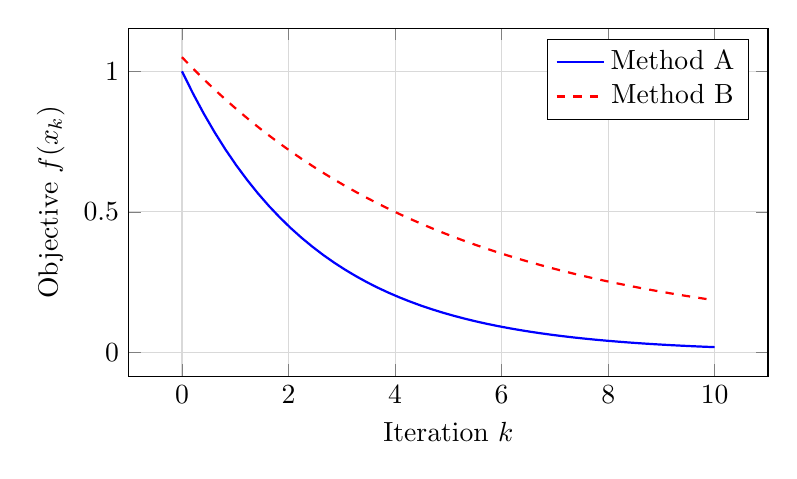
\begin{tikzpicture}
    \begin{axis}[
        width=0.8\textwidth,
        height=6cm,
        xlabel={Iteration $k$},
        ylabel={Objective $f(x_k)$},
        legend pos=north east,
        grid=both,
        grid style={gray!30},
      ]
      \addplot[blue, thick, domain=0:10, samples=50] {exp(-0.4*x)};
      \addlegendentry{Method A}
      \addplot[red, thick, dashed, domain=0:10, samples=50] {exp(-0.2*x) + 0.05};
      \addlegendentry{Method B}
    \end{axis}
  \end{tikzpicture}
  \caption{Convergence of the objective function for two methods.}
  \label{fig:convergence}
\end{figure}

\subsection{Architecture}

\Cref{fig:architecture} depicts the build pipeline that produced this
document.

\begin{figure}[htbp]
  \centering
  \begin{tikzpicture}[
      node distance=2.2cm,
      box/.style={rectangle, draw, rounded corners, minimum width=2.6cm,
                  minimum height=1cm, align=center, fill=blue!8},
      arrow/.style={-{Stealth}, thick},
    ]
    \node[box] (src) {Paper sources\\ \small \texttt{papers/<name>/}};
    \node[box, right=of src] (zig) {Zig build\\ \small \texttt{build.zig}};
    \node[box, right=of zig] (mk) {\texttt{latexmk}\\ \small multi-pass};
    \node[box, right=of mk] (pdf) {PDF\\ \small \texttt{zig-out/<name>.pdf}};
    \draw[arrow] (src) -- (zig);
    \draw[arrow] (zig) -- (mk);
    \draw[arrow] (mk) -- (pdf);
  \end{tikzpicture}
  \caption{The Zig build pipeline for a paper.}
  \label{fig:architecture}
\end{figure}
